\section{Benutzerhandbuch}
\subsection{Einleitung}

Das Digital Input Computer Keyboard ist eine Art elektronisches Keyboard, dass verschiedene Samples abspielen und aufnehmen kann. Man kann mithilfe der gegebenen Samples (Piano und Schlagzeug) spielen und Tonspuren aufnehmen. Aufgenommene Tonspuren können dann auch parallel abgespielt werden. Es können aber auch eigene Samples in das Programm geladen werden. Mit diesen kann man ebenso verfahren wie mit den gegebenen.

\begin{figure}[hbtp]
\centering
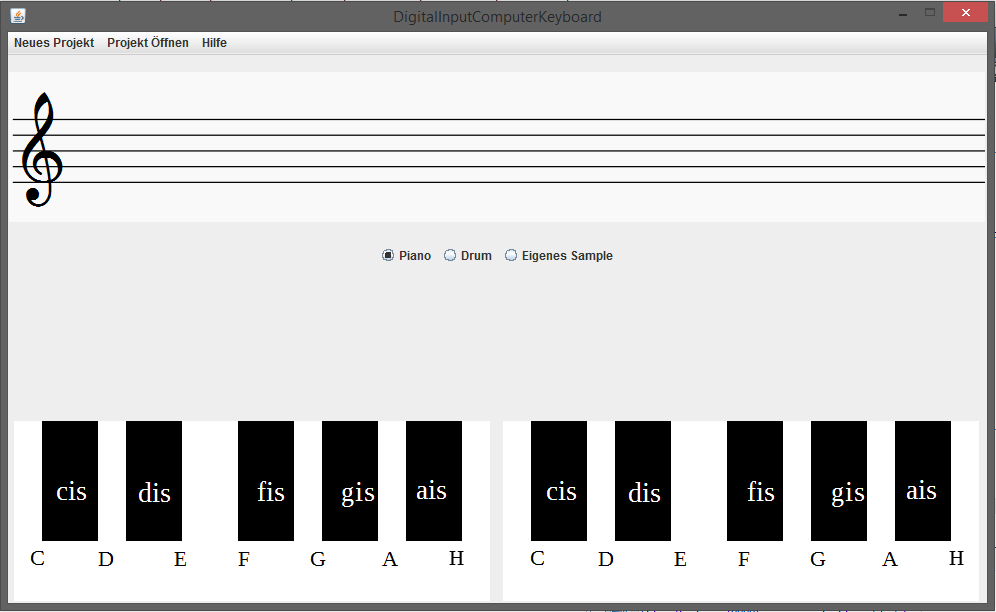
\includegraphics[scale=0.4]{Bilder/Projektbild1.PNG} 
\caption{Bild der Benutzeroberfläche}
\end{figure}


\subsection{Projekt}

Mithilfe des DICKs hat man die Möglichkeit Projekte zu erstellen. Ein Projekt enthält dann ein Projektfile, einen Ordner in dem eigene Aufnahmen abgespeichert sind und einen Sample Ordner in den man eigene Samples hinein laden kann.

\newpage


\subsubsection{Erstellen}

Mithilfe des Buttons "Neues Projekt" kann man einen Projekt Ordner erstellen. Dieser Ordner muss erst benannt und dann ein Speicherort ausgewählt werden. Während der Namensgebung aktivieren sich die Tasten, dies kann aber ignoriert werden. Sobald der Ordner erstellt wurde kann man einfach die Meldungen wieder schließen.

\begin{figure}[hbtp]
\centering
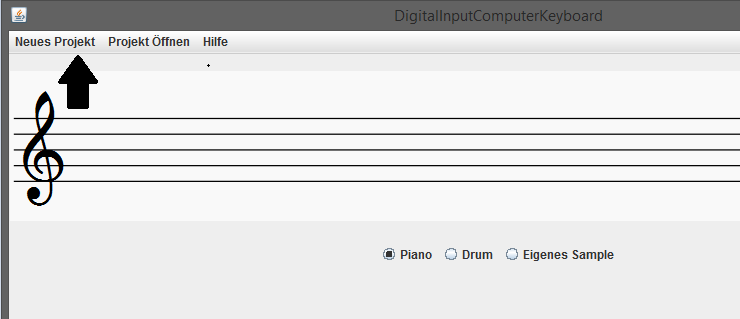
\includegraphics[scale=0.6]{Bilder/Projektbild2_1.PNG}
\caption{Der Button Neues Projekt}
\end{figure}


\subsubsection{Öffnen}

Wenn man bereits ein Projekt erstellt hat kann man dieses mithilfe des Buttons "Projekt Öffnen" öffnen. Man sucht den Projekt Ordner und wählt die Projektfile.bin aus. Sobald dies erledigt wurde, öffnet sich ein separates Fenster in dem man weitere Funktionen zur Auswahl hat.

\begin{figure}[hbtp]
\centering
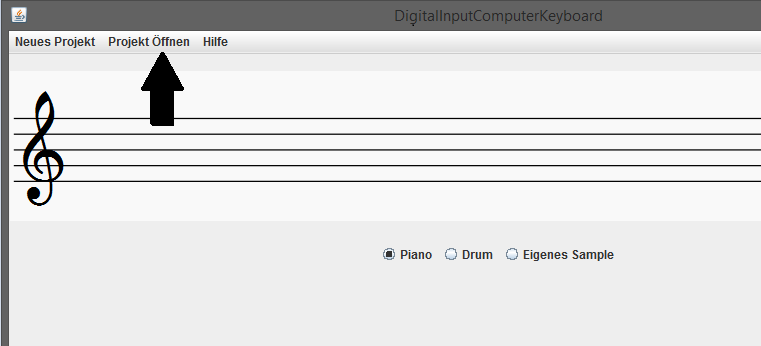
\includegraphics[scale=0.6]{Bilder/Projektbild3_1.PNG}
\caption{Der Button Projekt Öffnen}
\end{figure}

\newpage




\subsubsection{Aufnehmen}

Sobald man ein Projekt erstellt und geöffnet hat, kann man gespieltes Aufnehmen. Dazu muss man das Tempo und den Namen der Datei eingeben die aufgenommen werden soll. Zu beachten ist hierbei dass man sobald der Name oder das Tempo eingegeben wurde Enter gedrückt wird, da diese während dem spielen sonst verändert werden.









\subsubsection{Abspielen}

Um ein aufgenommenes Sample abzuspielen betätigt man den Abspielen Button. Dadurch öffnet sich ein Fenster in dem man seine aufgenommenen Samples sieht. Durch Auswahl eines Szenarios wird ein Fenster geöffnet das einen Button enthält. Durch betätigen des Buttons wird das Sample abgespielt. Dabei werden die aufgenommenen Noten angezeigt. 



\subsubsection{Eigene Samples}
 8oder16 bit wav  name 
 
 Um eigene Samples in das Programm einzufügen muss man diese in den Sample Ordner des Projekt einfügen. Dabei muss man einige Dinge beachten:
 
 \begin{itemize}
   \item[•] Die Töne des Samples müssen 8 oder 16 bit lang sein.
   \item[•] Es müssen wav Dateien sein.
   \item[•] Die Töne müssen wie folgt bezeichnet sein:
   	
   
 \end{itemize}            
             
             
             
             
             
             
             
             
             
             
             
             
             
             
             